% Options for packages loaded elsewhere
\PassOptionsToPackage{unicode}{hyperref}
\PassOptionsToPackage{hyphens}{url}
%
\documentclass[
]{article}
\usepackage{lmodern}
\usepackage{amssymb,amsmath}
\usepackage{ifxetex,ifluatex}
\ifnum 0\ifxetex 1\fi\ifluatex 1\fi=0 % if pdftex
  \usepackage[T1]{fontenc}
  \usepackage[utf8]{inputenc}
  \usepackage{textcomp} % provide euro and other symbols
\else % if luatex or xetex
  \usepackage{unicode-math}
  \defaultfontfeatures{Scale=MatchLowercase}
  \defaultfontfeatures[\rmfamily]{Ligatures=TeX,Scale=1}
\fi
% Use upquote if available, for straight quotes in verbatim environments
\IfFileExists{upquote.sty}{\usepackage{upquote}}{}
\IfFileExists{microtype.sty}{% use microtype if available
  \usepackage[]{microtype}
  \UseMicrotypeSet[protrusion]{basicmath} % disable protrusion for tt fonts
}{}
\makeatletter
\@ifundefined{KOMAClassName}{% if non-KOMA class
  \IfFileExists{parskip.sty}{%
    \usepackage{parskip}
  }{% else
    \setlength{\parindent}{0pt}
    \setlength{\parskip}{6pt plus 2pt minus 1pt}}
}{% if KOMA class
  \KOMAoptions{parskip=half}}
\makeatother
\usepackage{xcolor}
\IfFileExists{xurl.sty}{\usepackage{xurl}}{} % add URL line breaks if available
\IfFileExists{bookmark.sty}{\usepackage{bookmark}}{\usepackage{hyperref}}
\hypersetup{
  pdftitle={ECON 340 Homework 1},
  pdfauthor={Victor A. Tran},
  hidelinks,
  pdfcreator={LaTeX via pandoc}}
\urlstyle{same} % disable monospaced font for URLs
\usepackage[margin=1in]{geometry}
\usepackage{longtable,booktabs}
% Correct order of tables after \paragraph or \subparagraph
\usepackage{etoolbox}
\makeatletter
\patchcmd\longtable{\par}{\if@noskipsec\mbox{}\fi\par}{}{}
\makeatother
% Allow footnotes in longtable head/foot
\IfFileExists{footnotehyper.sty}{\usepackage{footnotehyper}}{\usepackage{footnote}}
\makesavenoteenv{longtable}
\usepackage{graphicx,grffile}
\makeatletter
\def\maxwidth{\ifdim\Gin@nat@width>\linewidth\linewidth\else\Gin@nat@width\fi}
\def\maxheight{\ifdim\Gin@nat@height>\textheight\textheight\else\Gin@nat@height\fi}
\makeatother
% Scale images if necessary, so that they will not overflow the page
% margins by default, and it is still possible to overwrite the defaults
% using explicit options in \includegraphics[width, height, ...]{}
\setkeys{Gin}{width=\maxwidth,height=\maxheight,keepaspectratio}
% Set default figure placement to htbp
\makeatletter
\def\fps@figure{htbp}
\makeatother
\setlength{\emergencystretch}{3em} % prevent overfull lines
\providecommand{\tightlist}{%
  \setlength{\itemsep}{0pt}\setlength{\parskip}{0pt}}
\setcounter{secnumdepth}{-\maxdimen} % remove section numbering

\title{ECON 340 Homework 1}
\author{Victor A. Tran}
\date{2/5/2020}

\begin{document}
\maketitle

\hypertarget{amazon-example-options-summary}{%
\section{Amazon Example Options
Summary}\label{amazon-example-options-summary}}

Which option is the best deal for me as a borrower?
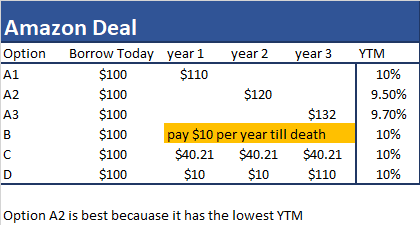
\includegraphics{C:/Users/victor/Desktop/Economics_R_Code/Images/HW1_Amazon_Options.png}

\hypertarget{chapter-3-quantative-problems}{%
\section{Chapter 3 Quantative
Problems}\label{chapter-3-quantative-problems}}

\hypertarget{problem-3}{%
\subsubsection{Problem 3}\label{problem-3}}

\begin{center}\rule{0.5\linewidth}{\linethickness}\end{center}

Consider a bond with a 7\% annual coupon and a face value of \$1000.
Complete the following table:

\begin{longtable}[]{@{}ccc@{}}
\toprule
Years to Maturity & Years to Maturity & Current Price\tabularnewline
\midrule
\endhead
3 & 5 & 1054\tabularnewline
3 & 7 & 1000\tabularnewline
6 & 7 & 1000\tabularnewline
9 & 7 & 1000\tabularnewline
9 & 9 & 880\tabularnewline
\bottomrule
\end{longtable}

\[\ Current Price (p) = \frac{70}{(1+0.05)^1} + \frac{70}{(1+0.05)^2} + \frac{70}{(1+0.05)^3} + \frac{1000}{(1+0.05)^3} = 1054   \]

\[\ Current Price (p) = \frac{70}{(1+0.07)^1} + \frac{70}{(1+0.07)^2} + \frac{70}{(1+0.07)^3} + \frac{1000}{(1+0.07)^3} = 1000   \]

\[\ Current Price (p) = \frac{70}{(1+0.07)^1} + \frac{70}{(1+0.07)^2} + \frac{70}{(1+0.07)^3} + \frac{70}{(1+0.07)^4} +\frac{70}{(1+0.07)^5} + \frac{70}{(1+0.07)^6} + \frac{1000}{(1+0.07)^6} = 1000   \]
\[\ Current Price (p) = \frac{70}{(1+0.07)^1} + \frac{70}{(1+0.07)^2} + \frac{70}{(1+0.07)^3} + \frac{70}{(1+0.07)^4} +\frac{70}{(1+0.07)^5} + \frac{70}{(1+0.07)^6} + \frac{70}{(1+0.07)^7} + \frac{70}{(1+0.07)^8} + \frac{70}{(1+0.07)^9} + \frac{1000}{(1+0.07)^9} = 1000   \]
\[\ Current Price (p) = \frac{70}{(1+0.09)^1} + \frac{70}{(1+0.09)^2} + \frac{70}{(1+0.09)^3} + \frac{70}{(1+0.09)^4} +\frac{70}{(1+0.09)^5} + \frac{70}{(1+0.09)^6} + \frac{70}{(1+0.09)^7} + \frac{70}{(1+0.09)^8} + \frac{70}{(1+0.09)^9} + \frac{1000}{(1+0.09)^9} = 880   \]
What relationship do you observe between maturity and discount rate and
the current price?

First, when the coupon rate = YTM, then the price of the bond = the face
value/ current price of the bond. Second, there is a negative
correlation between YTM and bond price. As YTM increase, price decrease.

\hypertarget{problem-6}{%
\subsubsection{Problem 6}\label{problem-6}}

\begin{center}\rule{0.5\linewidth}{\linethickness}\end{center}

What is the price of a perpetuity that has a coupon of \$50 per year and
a yield to maturity (YTM) of 2.5\% ? If the YTM doubles, what will
happen to its price?

\[\ P_c = \frac{C}{i_C} = \frac{50}{0.025} = 2000 \] If YTM double, then
\[\ P_c = \frac{C}{i_C} = \frac{50}{0.5} = 1000 \] This shows that price
and YTM are negatively correlated and proportional, since when YTM
double, price was reduce by half.

\hypertarget{problem-8}{%
\subsubsection{Problem 8}\label{problem-8}}

\begin{center}\rule{0.5\linewidth}{\linethickness}\end{center}

Suppose that you want to take out a loan and that your local bank wants
to charge you an annual real interest rate equal to 3\%. Assuming that
the annualized expected rate of inflation over the life of the loan is
1\%, determine the nominal interest rate that the bank will charge you.
What was the actual real interest rate on the loan if, over the life of
the loan, actual inflation is 0.5\%?

Determining the nominal interest rate: \[\ i_n = i_r + \Pi^{e} \]
\[\ i_n = 0.03 + 0.01 = 0.04 \] nominal interest rate is 4\%

What if the the actual real interest rate on the loan if, over the life
of the loan, actual inflation is 0.5\% instead of 1\%?
\[\ i_n = i_r + \Pi^{e} \] \[\ 0.04 = i_r + 0.005 \]
\[\ i_r = 0.04 - 0.005 = 0.035  \] The bank will charge an annualized
real interest of 3.5\% instead \#\#\# Problem 9 *** Lucia just bought
two coupons, one with a face value of 1000, and the other with a face
value of 5000. Both bonds have a coupon rate of 5\% and sold at par
today. Calculate both bonds's current yield and both bond's rate of
return if Lucia is able to sell these bond one year late for \$100 more
than the buying price. Can you estimate what happened to the interest
rate over that year?

\begin{longtable}[]{@{}ccccclc@{}}
\toprule
\begin{minipage}[b]{0.05\columnwidth}\centering
Bond\strut
\end{minipage} & \begin{minipage}[b]{0.11\columnwidth}\centering
Coupon Rate\strut
\end{minipage} & \begin{minipage}[b]{0.10\columnwidth}\centering
Face Value\strut
\end{minipage} & \begin{minipage}[b]{0.13\columnwidth}\centering
current Yield\strut
\end{minipage} & \begin{minipage}[b]{0.12\columnwidth}\centering
Capital Gain\strut
\end{minipage} & \begin{minipage}[b]{0.14\columnwidth}\raggedright
Rate of Return\strut
\end{minipage} & \begin{minipage}[b]{0.17\columnwidth}\centering
Future Bond Price\strut
\end{minipage}\tabularnewline
\midrule
\endhead
\begin{minipage}[t]{0.05\columnwidth}\centering
A\strut
\end{minipage} & \begin{minipage}[t]{0.11\columnwidth}\centering
5\%\strut
\end{minipage} & \begin{minipage}[t]{0.10\columnwidth}\centering
1000\strut
\end{minipage} & \begin{minipage}[t]{0.13\columnwidth}\centering
0.05\strut
\end{minipage} & \begin{minipage}[t]{0.12\columnwidth}\centering
0.1\strut
\end{minipage} & \begin{minipage}[t]{0.14\columnwidth}\raggedright
0.15\strut
\end{minipage} & \begin{minipage}[t]{0.17\columnwidth}\centering
1100\strut
\end{minipage}\tabularnewline
\begin{minipage}[t]{0.05\columnwidth}\centering
B\strut
\end{minipage} & \begin{minipage}[t]{0.11\columnwidth}\centering
5\%\strut
\end{minipage} & \begin{minipage}[t]{0.10\columnwidth}\centering
5000\strut
\end{minipage} & \begin{minipage}[t]{0.13\columnwidth}\centering
0.05\strut
\end{minipage} & \begin{minipage}[t]{0.12\columnwidth}\centering
0.02\strut
\end{minipage} & \begin{minipage}[t]{0.14\columnwidth}\raggedright
0.07\strut
\end{minipage} & \begin{minipage}[t]{0.17\columnwidth}\centering
5100\strut
\end{minipage}\tabularnewline
\bottomrule
\end{longtable}

For bond A: coupon payment = (5\% of 1000) = \$50 Current yield or
\[\ i_c = \frac{50}{1000} = 0.05  \]

Capital gain or \[\ g = \frac{100}{1000} = 0.1 \]

rate of return = \[\ i_c + g = 0.05 + 0.1 = 0.15 \] Bond A would provide
a rate of return of 15\%

For bond B: coupon payment = (5\% of 5000) = \$250 Current yield or
\[\ i_c = \frac{250}{5000} = 0.05  \]

Capital gain or \[\ g = \frac{100}{5000} = 0.02 \]

rate of return = \[\ i_c + g = 0.05 + 0.02 = 0.07 \] Bond A would
provide a rate of return of 7\%

\hypertarget{problem-10}{%
\subsubsection{Problem 10}\label{problem-10}}

\begin{center}\rule{0.5\linewidth}{\linethickness}\end{center}

You have paid \$980.30 for an 8\% coupon with a face value of 1000 that
matures in five years. You plan on holding the bond for one year. If you
want to earn a 9\% rate of return on this investment, what price must
you sell the bond for? Is this realistic?

\[\ 0.09 = \frac{80 + x}{1000}\] \[\ 90 = 80 + x\] \[\ x = 10\]
\[980.3 + x => 980.3 + 10 = 990.3\]

I would need to sell the bond for at least \$990.30 after the 1 year to
get a return rate of 9\%

\end{document}
